%[prl] it will mess up section numbers but puts our emails in the bibliography section
%[eqsecnum] Number equations by section
%
%
%\documentclass[prd,preprint,letterpaper]{revtex4}
%[nobibnotes],[nofootinbib]
\documentclass[aps,prb,twocolumn,superscriptaddress]{revtex4-1}

\usepackage{graphicx}	% this is the up-to-date package for all figures
\usepackage{amssymb}	% for math
\usepackage{verbatim}	% for the comment environment
\usepackage{color}
\usepackage{subcaption}	% for sub-captions on side-by-side figures
\usepackage{float}		% allows use of 'H' command
\usepackage{tikz}		% lets you draw: graphics, flowcharts, pie graphs, etc
\usepackage{footmisc} % to use footref, multiple footnotes referring to same thing
%\usepackage[final]{pdfpages}	% allows extern pdf to be included
\usetikzlibrary{arrows}

%%%
% For fancy section references
%%% 
% This allows you to use '\cref{}' to reference sections with the symbol
\usepackage{cleveref}
\crefname{section}{\S}{\S\S}%{§}{§§}
%% Usual (decimal) numbering
\renewcommand{\thesection}{\arabic{section}}
\renewcommand{\thesubsection}{\thesection.\arabic{subsection}}
\renewcommand{\thesubsubsection}{\thesubsection.\arabic{subsubsection}}
%% Fix references
\makeatletter
\renewcommand{\p@subsection}{}
\renewcommand{\p@subsubsection}{}
\makeatother
%%%%%
%%%


\def\deg{\ifmmode^\circ\else$^\circ$\fi}
\def\arcsec{\ifmmode^{\prime\prime}\else$^{\prime\prime}$\fi}
\def\arcmin{\ifmmode^{\prime}\else$^{\prime}$\fi}
\def\solar{\ifmmode_{\mathord\odot}\else$_{\mathord\odot}$\fi}
\def\earth{\ifmmode_{\mathord\oplus}\else$_{\mathord\oplus}$\fi}

%%%
% Change labeling of figures and tables - currently it defaults to 'FIG.'
%%%
\renewcommand{\figurename}{Figure}
\renewcommand{\thefootnote}{\roman{footnote}} %for footnotes in roman numerals
%\renewcommand{\thetable}{\Roman{table}}

\bibliographystyle{apsrev}


% these are some custom control of the page size and margins
% \topmargin= 0.2in  % these 1st two may be needed for some computers
% \textheight=8.75in
\textwidth=6.5in
%\oddsidemargin=0cm
%\evensidemargin=0cm


\begin{document}

\title{Assassinating ASASSN:\\ Supernovae Identification Using ATLAS Data}

\author{Corey Mutnik}
\email{cmutnik@hawaii.edu}
\affiliation{Department of Physics \& Astronomy, \\
University of Hawaii at Manoa,\\
2505 Correa Rd, Honolulu, HI, 96822, USA}
\altaffiliation{ASTR 399}


\begin{abstract}
Using current data collection and reduction techniques, we plan to 
identify supernovae (SNe) faster and fainter than the All-Sky Automated 
Survey for Supernovae (ASASSN) team.  
We expect to identify all SNe down to magnitudes of 17.5, with declinations 
(Dec) above $-30\deg$, before ASASSN.  
Over the course of four nights, ATLAS images each spot on the sky a minimum of five times.  
With a minimum of five observations per night of each object, it is possible to achieve 
magnitudes as low as 18.5.  
In the ATLAS pipeline, images are collected, reduced, and differenced.  To generate difference 
images, a composite image (wallpaper) is subtracted from the reduced images.   
Stationary transients stand out in difference images, increasing their probability of detection.  
Once images are differenced, certain restrictions are needed to distinguish between 
SNe and other real objects.  To differentiate between SNe and asteroids, multiple 
observations must be taken at the same position.  To eliminate variable stars, light curves 
must be constructed and analyzed.  Unlike variable stars, the light curve of SNe will not 
be periodic, it will contain only one node.
\end{abstract}


\maketitle    



\section{Introduction}
Observation of supernovae (SNe) is important in determining the distances of remote 
galaxies.  Type Ib and Ic supernovae have been shown to vary greatly in peak brightness, 
but type Ia supernova (SNIa) share the same magnitude (m) at the time of peak brightness.  
For this reason SNIa are commonly referred to as ``standard candles.''  This is 
an important feature, allowing for the calculation of distances to remote galaxies.  
Observing the violent outburst of a supernova (SN) gives us insight into our universe, 
as it was when the explosion occurred.  
Many cosmological questions are answered by SNe observations.  Based on the current 
data, we know the universe is expanding at an accelerated rate.  Another vital 
function of SN explosions is the dispersion of heavy elements throughout the universe.  
Using Asteroid Terrestrial-impact Last Alert System (ATLAS) data, we plan to identify 
SNe, with a focus on SNIa, faster and fainter than All-Sky Automated Survey for Supernovae 
(ASASSN).


\section{Collected Data}

\subsection{ASASSN Data}

\indent The All-Sky Automated Survey for Supernovae (ASASSN) group 
collects data using eight 14~cm telescopes. Each night, these  
telescopes are able to cover roughly 20,000~deg$^2$, reaching 
down to $\sim$17th magnitude.  
These eight telescopes are split evenly between two sites.  
The first telescope array is located on Haleakala and began 
collecting data in Dec 2013. In Jul 2015, the second %telescope 
array became operational at the LCOGT Cerro Tololo station.  
This allows ASASSN to detect SNe in both 
hemispheres~\cite{asn_data}.\\
\indent Using 400~mm f/2.8G Nikon lenses allows for a large field of 
view, while ProLine PL230 CCD cameras are used as detectors. Detection of 
transients is made possible using image subtraction. With images 
having 7.8\arcsec\ pixels, ASASSN relies on volunteers collecting  
confirmation images with larger 
telescopes.~\footnote{\label{foot:asn} http://www.astronomy.ohio-state.edu/ $\sim$assassin/index.shtml}



\begin{figure*}
	\centering
	\begin{subfigure}{.5\textwidth}
	  \centering
	  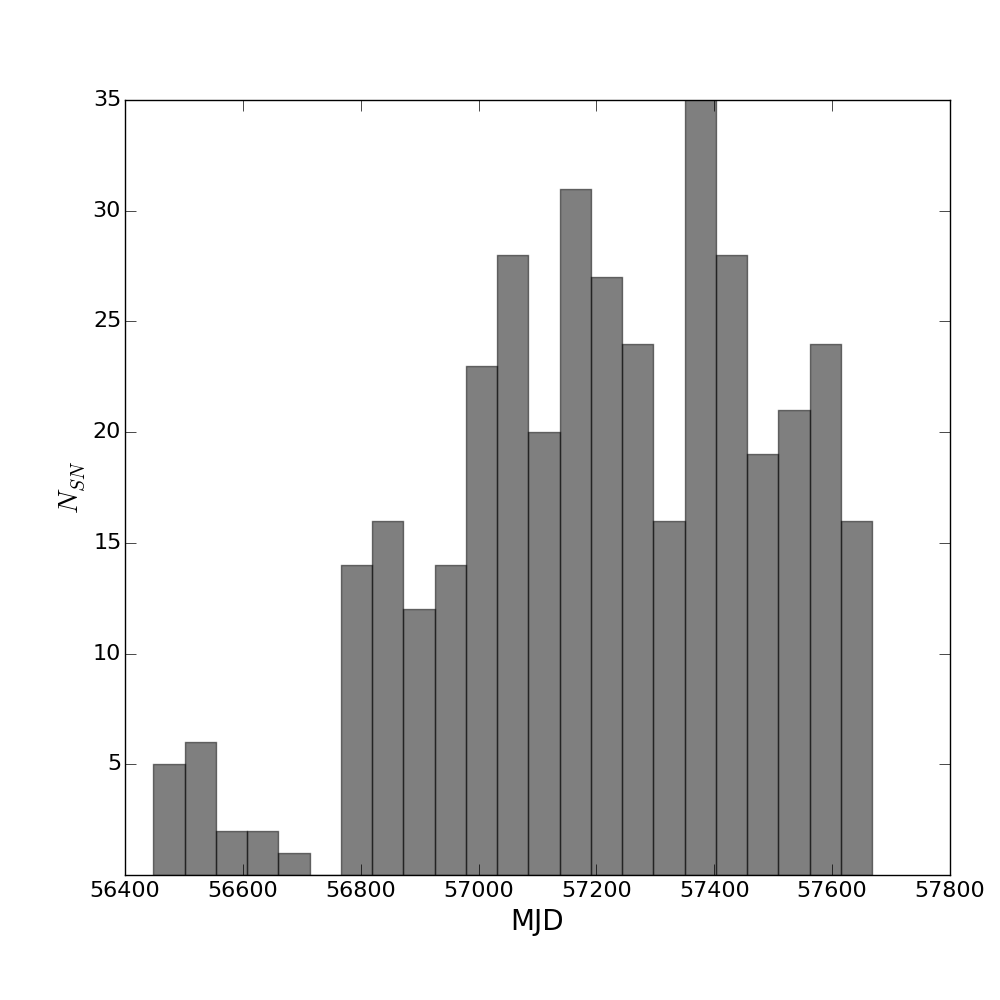
\includegraphics[width=1\linewidth]{figures/peak_mjd_histo_step50.png}
		\caption{\it \small{ }}
		\label{fig:mjdhist}
	\end{subfigure}%
	\begin{subfigure}{.5\textwidth}
	  \centering
			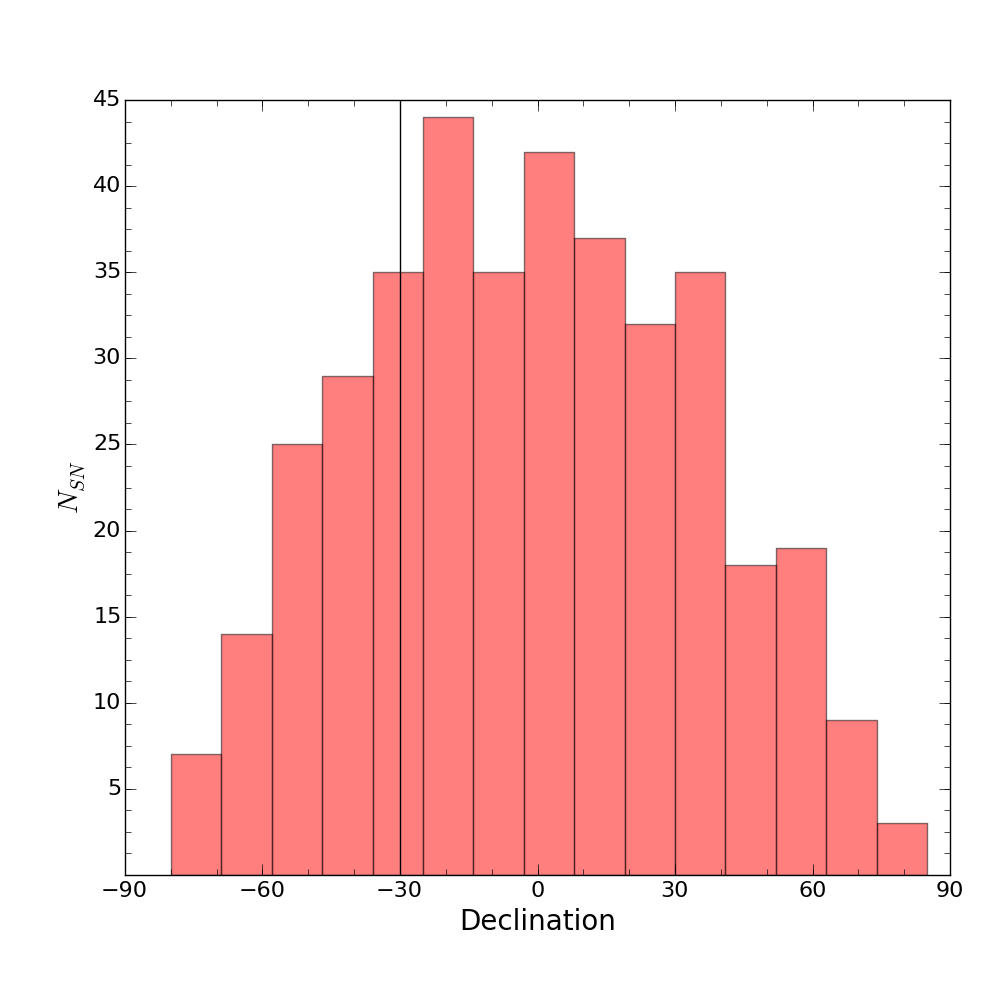
\includegraphics[width=1\linewidth]{figures/dec_histo_step10.png}
		\caption{\it \small{ }}
		\label{fig:dechist}
	\end{subfigure}
	\caption{\it \small{SN discovered by the ASASSN project.  Panel `(a)' shows ASASSN SN peak brightness dates.  Panel `(b)' is ASASSN data, binned by Dec. The vertical line at $-30\deg$ indicates the lower limit on ATLAS observations.}}
	\label{fig:asnhist}
\end{figure*}


\subsection{ATLAS}
ATLAS is a project funded by NASA to find dangerous asteroids.  The 
motivation and science justification was described by~\cite{ATLAS_data}.  
For the duration of this ASASSN project, ATLAS used an f/2, 0.5~m 
Schmidt telescope on Haleakala and a 110~Mpixel detector to collect 
30~deg$^2$ with each exposure.  This telescope was installed in Jun 
2015, and achieved more or less continuous operation around Sep 2015.  

ATLAS will shortly install a second telescope on Mauna Loa, and a 
proposal to NASA is being evaluated to build two more units for the 
southern hemisphere.

The pixel size is 1.86\arcsec\ and the field of view is
5.4$\times$5.4~deg.  The PSF is currently no better than 6.5\arcsec\
which degrades the limiting sensitivity by one magnitude.  The faulty
Schmidt corrector will be replaced in Mar 2017.  ATLAS uses two
filters ``$o$'' (essentially $r+i$) and ``$c$'' (essentially $g+r$),
changing according to the phase of the moon.

With the basic observation consisting of a 30~sec exposure and about 
13~sec of overhead, about 900 observations are collected per night.  
The observation strategy has varied since the telescope was 
installed, but currently observes one of four declination (Dec) bands between $-30$ 
and $+60$ Dec, imaging each spot 5 times on a $\sim$15~min cadence. 
The overlap between observations is about 0.4~deg, and they are 
dithered by a random amount for a given night, so each objects is seen 
5 or more times, depending on whether it falls in an overlap.  
Prior to Apr 2016, ATLAS collected 4 or more observations of each object 
per night. Increasing the number of observations per night from 4 to 5, 
while maintaining the same 4 day cadence, required an upper limit to 
be placed at a $+60$ Dec. This is shown by the dark gray region in 
the upper right hand corner of Figure~\ref{fig:dec_mjd}. 

The observations are processed by the ATLAS pipeline which consists of 
image flattening, star finding, star identification, high precision 
fits to astrometry (typically RMS of 0.3\arcsec\ per star and more 
than 10,000 stars) and photometry (typically 0.1~mag~RMS, limited by 
the current reference catalog), image differencing against a static sky 
image, and detection of objects that have moved or changed.  
Difference imaging and the detection of changing objects 
are discussed in~\cref{sec:diffimg}.


\subsubsection{Difference Imaging}\label{sec:diffimg}

Difference images are generated by subtracting the wallpaper from reduced 
images. This is done to isolate objects that are changing, as shown in 
Figure~\ref{fig:compreddiff}.  Figures~\ref{fig:red16ke} and \ref{fig:diff16ke} 
are reduced and difference images, respectively, of the SN ``ASASSN-16ke.''  
Subtraction of a properly calibrated wallpaper will produced a difference 
image containing only objects that are changing in the reduced images.  
After subtraction of the wallpaper, the SN is much more easily detected. 

The ``wallpaper'' (static sky image) is the weighted sum of many 
observations at each point in the sky.  ATLAS currently uses the 
Alard algorithm~\cite{Alard_algorithm} for differencing, and the 
differences are dominated by photon noise and by systematics from 
saturated stars or flare artifacts from the Schmidt corrector.

\begin{figure*}
  \centering
  \begin{subfigure}{.5\textwidth}
    \centering
    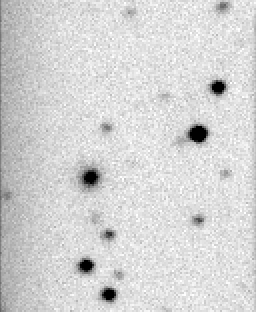
\includegraphics[width=0.5\linewidth]{figures/compare/red_ASASSN-16ke.png}
    \caption{\it \small{ }}
    \label{fig:red16ke}
  \end{subfigure}%
  \begin{subfigure}{.5\textwidth}
    \centering
      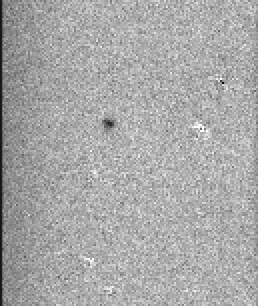
\includegraphics[width=0.5\linewidth]{figures/compare/diff_ASASSN-16ke.png}
    \caption{\it \small{ }}
    \label{fig:diff16ke}
  \end{subfigure}
  \caption{\it \small{Comparison between reduced and differenced images.  Panel `(a)' shows a reduced image containing the SN ``ASASSN-16ke.''  Panel `(b)' shows the same SN, but in a difference image.}}
  \label{fig:compreddiff}
\end{figure*}

The ATLAS mission is to find moving objects, but our processing
automatically finds all stationary transients and variable stars as
well.  Once the image is differenced, the program tphot detects all
sources at 3-sigma, and cut that back to 5-sigma once each source
has been fitted and the detection significance is known.  
This is augmented by calculated RA, Dec, magnitudes, and other relevant
quantities into a ``ddt'' (difference detection table) file.

\begin{figure}[h!]%[H]
 \resizebox{3in}{!}{%
 \tikzset{
  treenode/.style = {align=center, inner sep=1pt, font=\sffamily},
  arn_m/.style = {treenode, rectangle, rounded corners=1mm, black,
  font=\sffamily\bfseries, draw=black, minimum width=7em},
  arn_n/.style = {treenode, rectangle, black, font=\sffamily\bfseries, draw=black, minimum width=2em},
  arn_r/.style = {treenode, rectangle, black, draw=black, minimum width=3em, very thick},
  arn_x/.style = {treenode, rectangle, draw=black, minimum width=0.5em, minimum height=0.5em}
 }
 \begin{tikzpicture}[->,>=stealth',level/.style={sibling distance = 2.5cm/#1,
  level distance = 1cm}] 
 \node [arn_m] {Detections}
    child{ node [arn_r] {Real} 
            child{ node [arn_n] {Asteroid} edge from parent node[above left]
                    {$moving$}%for a named pointer
            }
            child{ node [arn_n] {Var}}
            child{ node [arn_n] {ST}}
    }
    child{ node [arn_r] {(Other)}
    }
    child{ node [arn_r] {Artifact}   
            child{ node [arn_n] {Star Scar}}
            child{ node [arn_n] {CR}}
            child{ node [arn_n] {Burn}}
            child{ node [arn_n] {xtalk}}                         
    }
 ; 
 \end{tikzpicture}%
 }%
 \caption{\it \small{Object classification probability flowchart.  Asteroids are real objects that are moving, ST stands for stationary transient, Var is variable star. Artifacts arise during image processing and are not real objects.\label{fig:probflow}}}
\end{figure}

The most useful classification variable is ``starrat'' (star ratio), 
which is defined to be the ratio of flux on the original, un--subtracted 
image to flux on the difference image.  Both fluxes are measured using a 
circular aperture of 2.0~pixel radius.  The star ratio is used in 
determining if an object is real or just a residuals from subtracted stars.  
For these, the star ratio will be large (usually greater than 5) because 
the star was much brighter before it was subtracted.  For asteroids and 
supernovae, we expect the star ratio to be near 1.0.  Since they are not 
usually in their recorded locations, such objects should not show up in the wallpaper.  
Any object that isn't in the wallpaper is left unchanged by difference imaging.  
This means the recorded flux to be the same both before and after image subtraction, 
resulting in starrat=1.0.  Figure~\ref{fig:starrat} shows the distribution of starrat 
values for all objects observed on the night of 57680.  SNe are located in the 
tight cluster around starrat=1.0.

\begin{figure}[h!]%[H]
\begin{center}
    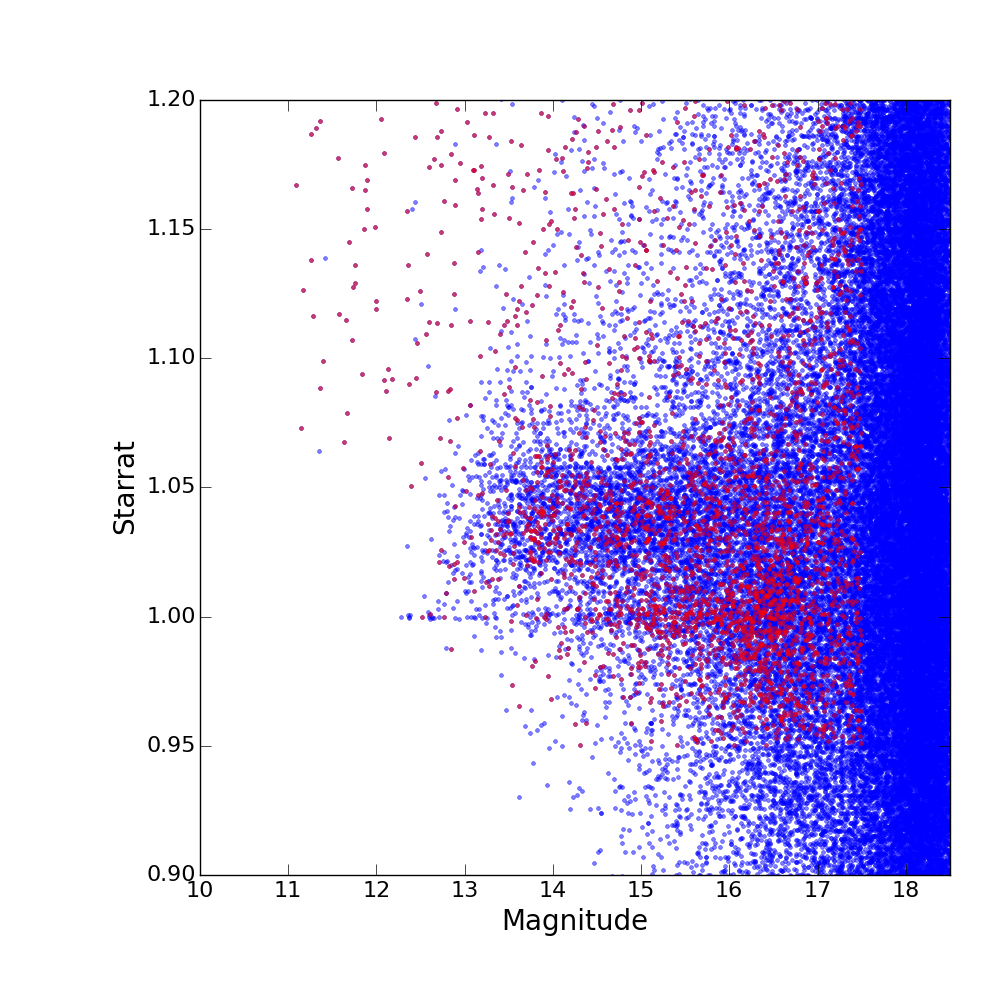
\includegraphics[width=1\linewidth]{figures/Starrat_mag_low_alpha0tac5_remake.png}%
     \caption{\it \small{57680 is used as an example to show the distribution of starrat as a function of magnitude.  Starrat values for all objects observed that night are shown in blue.  Shown in red, good SNe were isolated after applying classification restrictions.~\label{fig:starrat}}}
  \end{center}
\end{figure}

Difficulties include cases where a real transient can produce a high 
starrat, and cases where a false detection from a star residual can 
produce a low starrat. The former arise from the fact that supernovae 
happen in galaxies, which do get subtracted and can raise starrat 
substantially above 1.0 if they are bright. The latter can occur when 
we have a star residual detection substantially off-center from the 
star, so the flux on the un--subtracted image is not as bright as we might 
expect, and starrat can be lowered to the 2-5 range, or in some odd 
cases can be negative. So starrat is not foolproof. Nevertheless, a 
starrat value near 1.0, especially if accompanied by other indications 
such as consistent astrometry, is a useful piece of evidence pointing 
toward a real SN, asteroid, or other interesting transient.


\section{Procedure}

\indent In order to assassinate ASASSN, it was necessary to show that ATLAS 
had the potential to find all of ASASSN discovered SNe.  
To do this, a list of all ASASSN discovered SNe was obtained~\cite{asn_data}.  
By Oct 11, 2016 ASASSN has reported discovering 385 SNe. Many of these 
objects were reported before ATLAS was operation. Object cuts are discussed 
in~\cref{sec:expobs}. Once the data was properly culled, the remaining SNe 
were found in observations made by ATLAS.  
Finding these SNe in the ATLAS 
data allowed restrictions to be placed on classification variables, drastically 
reducing the number of potential SNe candidates. With such a restricted object 
list, visual examination is able to be used in identifying SNe.  It has been 
shown that all SNe can be detected using a star ratio between $0.9$ and $1.2$.


%%%%%%%%%%%%%%%%%%%%%%%%%%%%%%%%%%%%%%%%%%%%%%%%%%%%%%%%%%%%%%%%%%%%%%%%%%%%%%%%%%%%%%%%%%%%%%%%%%%%
%%%%%%%%%%%%%%%%%%%%%%%%%%%%%%%%%%%%%%%%%%%%%%%%%%%%%%%%%%%%%%%%%%%%%%%%%%%%%%%%%%%%%%%%%%%%%%%%%%%%
%%%
% input 2 sections: ``Expected Observations'' and ``Failed Matches''
%%%
\input sections/nocomment_section_expected_obs.tex
%%%%%%%%%%%%%%%%%%%%%%%%%%%%%%%%%%%%%%%%%%%%%%%%%%%%%%%%%%%%%%%%%%%%%%%%%%%%%%%%%%%%%%%%%%%%%%%%%%%%
%%%%%%%%%%%%%%%%%%%%%%%%%%%%%%%%%%%%%%%%%%%%%%%%%%%%%%%%%%%%%%%%%%%%%%%%%%%%%%%%%%%%%%%%%%%%%%%%%%%%



\section{Results and Discussion}

\indent Of the 385 SNe ASASSN discovered by Oct 2016, only 96 overlapped
with ATLAS in sky and time.  
In \cref{sec:expobs} and \cref{sec:failmatch} we discussed the 850 
ATLAS observations associated with the 96 SNe expected to be 
present in ATLAS data.  
It has been shown that all 96 ASASSN discovered SNe overlapping ATLAS 
observations in sky and time are detectable in ATLAS data.\\
%
\indent SNe discovered by ASASSN were used in refining ATLAS classification 
variables, such as starrat.  Variables like starrat reduce the 
false alarm rate by eliminating artifacts produced during image 
subtraction, as shown in Figure~\ref{fig:starrat}.  We verified all ASASSN 
SNe to have a starrat values between $0.9$ and $1.2$.  
Although using such a large starrat range would allow all SNe to be detected, 
it would also drastically increase the false alarm rate.  Further tests need 
to be conducted in order to find the optimal range for starrat; one that maximizes 
the number of SNe detected while minimizing the number of objects that need to be examined.  
Restricting classification variables drastically reduces the false alarm rate and leads 
to fewer objects needing visual inspection. This shows the ability 
for ATLAS to identify all SNe faster and fainter than ASASSN is able to.\\
%
\indent The detection of all SNIa between $-30$ and $+60$ Dec with 
magnitudes down to 17.5, is possible using ATLAS data.  
%As shown by Figure~\ref{fig:dec_mjd}, ATLAS was able to identify all of the SNe discovered by ASASSN
All SNe discovered by ASASSN, after ATLAS became truly operational, were 
able to be identified with ATLAS data alone.  This is shown in 
Figure~\ref{fig:dec_mjd}, with missed SNe falling on the edges of ATLAS 
observational limits.\\
%
\indent With a relatively short average lifespan, detection of a SNIa requires 
frequent coverage of the entire sky. Using current observation patterns,
ATLAS surveys the entire sky, between $-30$ and $+60$ Dec, in just 4 nights. 
Five observations of the entire sky are recorded by ATLAS every four nights, 
making it possible to detect SNIa down to magnitudes of 18.5.  During our analysis 
we ran successful tests down to m~$=18$.\\
%
\indent To differentiate between real objects 
and artifacts, we require objects to show up on 
more than one image collected during the night it was observed.  
This requirement drastically reduces our false alarm rate by 
eliminating artifacts such as star scars, as they 
are not consistently present.   
An object is determined to be real if it appears in all good 
observations overlapping that region of the sky.  
If an object appears in one of the images, it is expected to appear 
in the other overlapping images collected that night.  
Any object that appears in only one observation, it is deemed to be 
an artifact.  This simple criteria allows us to easily 
distinguish between artifacts and real objects.\\
%
\indent The final distinction that must be made is between the different 
types of real objects.  All real objects have defining characteristics.  
Asteroids and other non--stationary objects are not expected to be observed 
in the same position more than once.  Unlike moving objects, SNe are 
stationary transients; their position does not change as a function of time.  
To remove the possibility of an object being an asteroid, we require multiple 
observations be recorded at the same position.  In order to distinguish between 
SNe and other stationary transients, light curves must be constructed.  The light 
curve of a variable star will appear periodic, while that of a SNe will increase 
suddenly, then rapidly fall off.
%{\bf ~\\~[include comparison figure of LC's]}\\
%{\bf [in results section get into the range for starrat values]}\\


\section*{Acknowledgments}
I would like to thank \input ../acknowledgement.tex  % input acknowledgement




\setlength{\parindent}{0cm}

\bibliography{../biblio}

\end{document}
